\scanpage{15}
\[
(X^{\Delta_n})_0=\deleted{\underline{\operatorname{Hom}}}_B p_{B*}(\underline{\operatorname{Hom}}(p_A^*(\Delta_n),X))=X_n
\]
\[
(X^{\dot\Delta_n})_0=p_{B*}\underline{\operatorname{Hom}}(\dot\Delta_n,X)=\varprojlim(X_{n-1},X_{n-2})
\]
\diagram{\begin{tikzcd}X^{\Delta_n}\arrow[r]&X^{\dot\Delta_n}\times_{Y^{\dot\Delta_n}}Y^{\Delta_n}\end{tikzcd}}
\margin{$(\operatorname{cosk}_{n-1}X)_n\deleted{\unsure{X_2}}$}
\figure{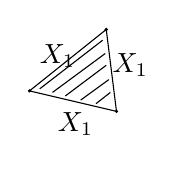
\begin{tikzpicture}[scale=.65]
\draw (0,0)--(1.5,1.2)--(1.7,-.4)--cycle;
\fill (0,0) circle(1pt);\fill(1.5,1.2)circle(1pt);\fill(1.7,-.4)circle(1pt);
\draw (.2,.04)--(1.43,.99) (.45,-.03)--(1.48,.73) (.7,-.1)--(1.5,.5) (1,-.18)--(1.55,.22) (1.3,-.25)--(1.58,-.03);
\node at(.55,.68){$X_1$};\node at(1.97,.5){$X_1$};\node at(.9,-.65){$X_1$};
\end{tikzpicture}}
\diagram{\begin{tikzcd}X_n\arrow[r]&(X^{\dot\Delta_n})_0\times_{(Y^{\dot\Delta_n})_0}Y_n\end{tikzcd}}
\margin{$A_n=A$\par $A$}
\diagram{\begin{tikzcd}X_{n-2}\arrow[r,no head,shift left=3]\arrow[r,no head]\arrow[r,no head,shift right=3]&X_{n-1}\end{tikzcd}}
\[\underline{\operatorname{Hom}}(\dot\Delta_n,a)\]
\diagram{\begin{tikzcd}\underline{\operatorname{Hom}}(M,a)\arrow[r,Rightarrow,"??"]&a\end{tikzcd}}
\[\operatorname{Hom}(X\times M,a)\simeq\operatorname{Hom}(X,-)\]
\[\operatorname{Hom}(\alpha\boxtimes(\beta\times M),\deleted{a}\unsure{a}\boxtimes e_B)\simeq\operatorname{Hom}(\alpha\boxtimes\beta,a\boxtimes\unsure{e_B}\]
\[\operatorname{Hom}\]
\[L\]
\figure{\begin{tikzpicture}[x=.075cm,y=.22cm]
\node[anchor=base west,inner sep=0pt,font=\tiny\ttfamily] at (0,0) {00040\ //ETAP1\ EXEC\ PGM=FLIPFLOP};
\node[anchor=base west,inner sep=0pt,font=\tiny\ttfamily] at (0,-1) {00050\ //SYSUT1\ DD\ DSN=CNU1.MODULEF.V33.INTERME1(MEFCOSDS),DISP=(OLD,PASS)};
\node[anchor=base west,inner sep=0pt,font=\tiny\ttfamily] at (0,-2) {00060\ //SYSUT2\ DD\ DSN=\&AUX,SPACE=(CYL,24),UNIT=SYSDA,DISP=(,PASS),};
\node[anchor=base west,inner sep=0pt,font=\tiny\ttfamily] at (0,-3) {00070\ //\ DCB=(RECFM=F\inserted{B},LRECL=80,BLKSIZE=\deleted{80}\inserted{19040})};
\node[anchor=base west,inner sep=0pt,font=\tiny\ttfamily] at (0,-4) {00080\ //ETAP2\ EXEC\ PGM=UPDATE,PARM=NEW,COND=(0,NE,ETAP1)};
\node[anchor=base west,inner sep=0pt,font=\tiny\ttfamily] at (0,-5) {00070\ //SYSPRINT\ DD\ DUMMY};
\node[anchor=base west,inner sep=0pt,font=\tiny\ttfamily] at (0,-6) {00100\ //SYSIN\ DD\ DSN=\&AUX,DISP=(OLD,DELETE)};
\node[anchor=base west,inner sep=0pt,font=\tiny\ttfamily] at (0,-7) {\deleted{00110\ //SYSIN2\ DD\ UNIT=SYSDA,SPACE=(CYL,24)}};
\node[anchor=base west,inner sep=0pt,font=\tiny\ttfamily] at (0,-8) {00120\ //SYSUT2\ DD\ DSN=CNU2.MODULEF.COSDS,};
\node[anchor=base west,inner sep=0pt,font=\tiny\ttfamily] at (0,-9) {00130\ //\ UNIT=SYSDA,DISP=(,CATLG,DELETE),SPACE=(TRK,(180,0,35),RLSE),};
\node[anchor=base west,inner sep=0pt,font=\tiny\ttfamily] at (0,-10) {00140\ //\ VOL=SER=SYS\unsure{PPP|PFP},DCB=(RECFM=FB,LRECL=80,BLKSIZE=19040)};
\node[anchor=base west,inner sep=0pt,font=\tiny\ttfamily] at (0,-11) {00150\ //COMP\ \ \ \ \ \ \ EXEC\ FORTXC,PARM=TERM,REGION=6000K};
\node[anchor=base west,inner sep=0pt,font=\tiny\ttfamily] at (0,-12) {00160\ //FORT.SYSPRINT\ DD\ DSN=\&MESSYS,UNIT=SYSDA,DISP=(MOD,PASS),};
\node[anchor=base west,inner sep=0pt,font=\tiny\ttfamily] at (0,-13) {00170\ //\ SPACE=(CYL,24)};
\node[anchor=base west,inner sep=0pt,font=\tiny\ttfamily] at (0,-14) {00180\ //FORT.SYSTERM\ DD\ DSN=\&MESCOM,UNIT=SYSDA,DISP=(MOD,PASS),};
\node[anchor=base west,inner sep=0pt,font=\tiny\ttfamily] at (0,-15) {00185\ //\ SPACE=(CYL,12)};
\node[anchor=base west,inner sep=0pt,font=\tiny\ttfamily] at (0,-16) {00190\ //SYSIN\ \ \ \ DD\ DSN=CNU1.MODULEF.V33.INTERME1(MEFCOSDS),DISP=OLD};
\node[anchor=base west,inner sep=0pt,font=\tiny\ttfamily] at (0,-17) {00200\ //CUTR\ \ \ \ EXEC\ PGM=CUTTER,COND=(0,NE,COMP.FORT)};
\node[anchor=base west,inner sep=0pt,font=\tiny\ttfamily] at (0,-18) {00210\ //TERMINAL\ DD\ DSN=\&MESCOM,DISP=(OLD,DELETE)};
\node[anchor=base west,inner sep=0pt,font=\tiny\ttfamily] at (0,-19) {00220\ //OBJECT1\ DD\ DSN=\&OBJ,DISP=(OLD,DELETE)};
\node[anchor=base west,inner sep=0pt,font=\tiny\ttfamily] at (0,-20) {00230\ //SOURCE1\ DD\ DSN=\&MESSYS,DISP=(OLD,DELETE)};
\node[anchor=base west,inner sep=0pt,font=\tiny\ttfamily] at (0,-21) {00240\ //SYSPRINT\ DD\ SYSOUT=*};
\node[anchor=base west,inner sep=0pt,font=\tiny\ttfamily] at (0,-22) {00250\ //SOURCE2\ DD\ DUMMY};
\node[anchor=base west,inner sep=0pt,font=\tiny\ttfamily] at (0,-23) {00260\ //OBJECT2\ DD\ DSN=\&OBJ2,SPACE=(CYL,24),UNIT=SYSDA,DISP=(MOD,PASS)};
\node[anchor=base west,inner sep=0pt,font=\tiny\ttfamily] at (0,-24) {00270\ //LIEN\ \ \ \ \ \ \ EXEC\ FORTXL,COND=((0,NE,COMP.FORT),(0,NE,CUTR)),};
\node[anchor=base west,inner sep=0pt,font=\tiny\ttfamily] at (0,-25) {00280\ //\ PARM=NCAL};
\node[anchor=base west,inner sep=0pt,font=\tiny\ttfamily] at (0,-26) {00290\ //LKED.SYSLIN\ DD\ DSN=\&OBJ2,DISP=(OLD,DELETE)};
\node[anchor=base west,inner sep=0pt,font=\tiny\ttfamily] at (0,-27) {00300\ //LKED.SYSLMOD\ DD\ DSN=CNU2.MODULEF.COSD,SPACE=(TRK,(180,0,35),RLSE),};
\node[anchor=base west,inner sep=0pt,font=\tiny\ttfamily] at (0,-28) {00310\ //\ DCB=(RECFM=U,BLKSIZE=19040),UNIT=SYSDA,VOL=SER=SYS\unsure{PPP|PFP}};
\node[anchor=base west,inner sep=0pt,font=\tiny\ttfamily] at (0,-29) {00320\ //\ DISP=(,CATLG,DELETE)};
\node[anchor=base west,inner sep=0pt,font=\tiny\ttfamily] at (0,-30) {00330\ //};

\draw[->,thick](-3,-3)--(-.5,-3);\draw[->,thick](-3,-4)--(-.5,-4);\draw[->,thick](-3,-7)--(-.5,-7);
\draw(28,-4)ellipse(3.5,.65);
\node[anchor=base west,font=\tiny] at(26,-4.7){\inserted{\unsure{IEBUPDTE}}};
\end{tikzpicture}}
\mspage{14}
